\section{Another Way to Describe a Point: Polar Coordinates}

The Cartesian description of a point uses two signed distances:

\[
P=(x,y).
\]

This is natural when horizontal and vertical directions are important. It is not,
however, the only possible way to describe position in the plane. We may instead
ask two different questions:

\begin{enumerate}
    \item How far is the point from the origin?
    \item In which direction do we move from the origin to reach it?
\end{enumerate}

These questions lead to \emph{polar coordinates}. A point is described by a pair

\[
(r,\theta),
\]

where $r\geq 0$ is the distance from the origin and $\theta$ is the angle measured
from the positive $x$-axis.

\begin{center}
\begin{tikzpicture}[scale=1.05]
    \draw[->] (-0.5,0) -- (4.8,0) node[right] {$x$};
    \draw[->] (0,-0.5) -- (0,3.8) node[above] {$y$};
    \coordinate (O) at (0,0);
    \coordinate (P) at (3.6,2.4);
    \draw[thick] (O) -- (P) node[midway,above left] {$r$};
    \draw[dashed] (P) -- (3.6,0);
    \draw[dashed] (P) -- (0,2.4);
    \draw (0.9,0) arc[start angle=0,end angle=33.69,radius=0.9];
    \node at (1.15,0.35) {$\theta$};
    \fill (P) circle (2pt) node[above right] {$P$};
    \fill (O) circle (1.5pt) node[below left] {$O$};
\end{tikzpicture}
\end{center}

The two descriptions refer to the same point. The right triangle in the figure
gives

\[
x=r\cos\theta,
\qquad
y=r\sin\theta.
\]

Conversely, if the Cartesian coordinates are known, then

\[
r=\sqrt{x^2+y^2}.
\]

The angle must be chosen so that its sine and cosine have the correct signs. For
this reason, the formula $\theta=\arctan(y/x)$ must be used with care: it does not
by itself distinguish all four quadrants.

\begin{examplebox}
Consider the point whose polar coordinates are

\[
(r,\theta)=\left(2,\frac{\pi}{3}\right).
\]

Its Cartesian coordinates are

\[
x=2\cos\frac{\pi}{3}=1,
\qquad
y=2\sin\frac{\pi}{3}=\sqrt{3}.
\]

Thus the same point may be written as

\[
P=\left(1,\sqrt{3}\right)
\]

in Cartesian coordinates and as

\[
P=\left(2,\frac{\pi}{3}\right)
\]

in polar coordinates.
\end{examplebox}

Polar coordinates are especially convenient when distance from the origin is the
main geometric feature. Let

\[
C_R
=
\{(x,y)\in\mathbb{R}^2:x^2+y^2=R^2\}.
\]

This is the set of all points in the Cartesian plane whose coordinates satisfy
the condition

\[
x^2+y^2=R^2.
\]

Geometrically, $C_R$ is the circle of radius $R$ centred at the origin.
After substituting

\[
x=r\cos\theta,
\qquad
y=r\sin\theta,
\]

the Cartesian condition becomes

\[
r^2\cos^2\theta+r^2\sin^2\theta=R^2.
\]

Since $\cos^2\theta+\sin^2\theta=1$, this reduces to

\[
\boxed{r=R}.
\]

The set $C_R$ has not changed. The conditions

\[
x^2+y^2=R^2
\qquad\text{and}\qquad
r=R
\]

describe the same geometric subset of the plane, but they use different
coordinates. In Cartesian coordinates we express a relation between horizontal
and vertical position. In polar coordinates we state directly that every point
of the set has the same distance from the origin.

\begin{center}
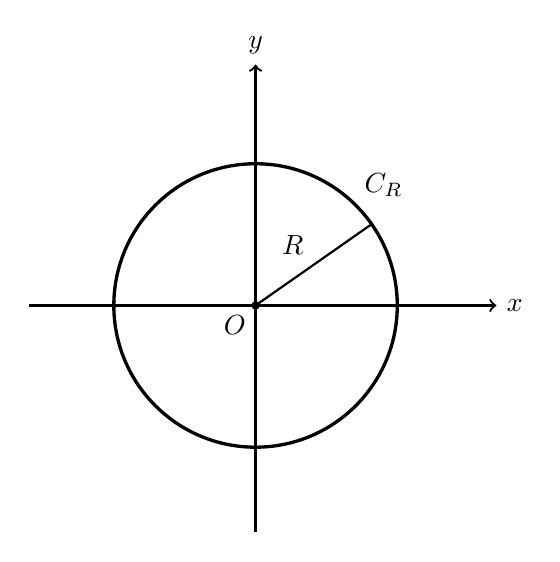
\begin{tikzpicture}[scale=0.9]
    \draw[->,thick] (-3.2,0) -- (3.4,0) node[right] {$x$};
    \draw[->,thick] (0,-3.2) -- (0,3.4) node[above] {$y$};
    \draw[very thick] (0,0) circle (2);
    \draw[thick] (0,0) -- ({2*cos(35)},{2*sin(35)})
        node[midway,above left] {$R$};
    \fill (0,0) circle (1.7pt) node[below left] {$O$};
    \node[above right] at (1.4,1.4) {$C_R$};
\end{tikzpicture}
\end{center}

\begin{remarkbox}
Polar coordinates are not unique. The angles $\theta$ and $\theta+2\pi$ describe
the same direction, so the pairs

\[
(r,\theta)
\qquad\text{and}\qquad
(r,\theta+2\pi)
\]

represent the same point in the plane. At the origin, where $r=0$, the angle is
irrelevant. This is a first example of an important distinction: a geometric
object may be unique even when its coordinate description is not.
\end{remarkbox}
